% !TEX root = B&G_oefeningen.tex
\chapter{Recursie}
In dit OPO bestuderen we twee speciale datastructuren: bomen en grafen. Omdat er hiervoor nogal veel recursief geprogrammeerd moet worden, is het zinvol om aan dit principe wat extra aandacht te besteden. Hieronder vind je de oefeningen van de eerste lesweek.
\begin{oef}
\code Implementeer een recursieve methode \verb/fibonacci(int getal)/ die het \verb/getal/-de fibonacci-getal berekent (zie \url{https://nl.wikipedia.org/wiki/Rij_van_Fibonacci}). Vermoedelijk vind je een eenvoudige en korte versie die echter heel inefficiënt is. Kan je uitleggen waarom? 
\begin{opl}
De defintie op Wikipedia klopt volgens ons niet helemaal. Het eerste Fibonaccigetal is niet 0, maar 1. Het tweede Fibonaccigetal is ook 1. Daarna is het n-de Fibonaccigetal gelijk aan de som van de twee vorige. De code in listing~\ref{recfibo} is kort, maar nogal onefficiënt. Om het 100ste getal te berekenen, moeten we eerst het 99ste en het 98ste getal berekenen en die optellen. Om het 99ste te berekenen moeten we echter opnieuw eerst het 98ste berekenen. We doen dus veel te veel werk.
\begin{lstlisting}[caption={Recursieve methode om Fibonacci-getallen te berekenen}, label=recfibo]
public static int fibonacci(int getal) {
	if (getal <= 0)
		throw new IllegalArgumentException();
	if (getal <= 2)
		return 1;
	else
		return fibonacci(getal - 1) + fibonacci(getal - 2);
}
\end{lstlisting}
\end{opl}

\end{oef}

\begin{oef}
\code Schrijf een recursieve methode \verb/somCijfers(int getal)/. Uitvoer is de som van de cijfers van \verb/getal/. 

Voorbeeld: 234 $\rightarrow$ $2+3+4=9$
\begin{opl}
\begin{lstlisting}[caption={Recursieve methode om de som van de cijfers van een getal te berekenen}, label=recsomgetallen]
public static int somVanCijfers(int getal) {
	getal = Math.abs(getal);
	if (getal < 10) //basisgeval, slechts 1 cijfer
		return getal;
	else //getal bestaat uit meer dan 1 cijfer, recursieve oproep van de functie nodig
		return getal % 10 + somVanCijfers(getal / 10);
}
\end{lstlisting}
\end{opl}

\end{oef}




\begin{oef}
\code Schrijf een recursieve methode \verb/keerOm(String str)/. Uitvoer is een string waarbij alle karakters van \verb/str/ in omgekeerde volgorde voorkomen.

Voorbeeld: \verb/abcd/ $\rightarrow$ \verb/ dcba/

{\textbf{Uitbreiding:}} Vind twee versies van het algoritme. In de eerste versie wordt de omgekeerde string van links naar rechts opgebouwd; in de tweede versie van rechts naar links.
\begin{opl}
Een vraag die we geregeld krijgen in de oefenzitting is waarom het niet werkt als de test of de gegeven string null is, later in de code staat, bvb. na de test of de lengte van de string kleiner of gelijk is aan 1. Wat gebeurt er als je de lengte vraagt van een niet bestaande string? In plaats van \verb+charAt+ kan je vanzelfsprekend ook gebruik maken van \verb+substring+. 
\begin{lstlisting}[caption={Recursieve methode om een string om te keren}, label=reckeerom]
public static String keerOm(String s) {
	if (s == null)
		throw new IllegalArgumentException();
	else if (s.length() <= 1)
		return s;
	else
		return s.charAt(s.length() - 1) + Recursie.keerOm(s.substring(0, s.length() - 1));
}
\end{lstlisting}
\end{opl}

\end{oef}

\begin{oef}
\code Implementeer een recursieve methode \verb/countX(String str)/. Invoer is de string \verb/str/. Uitvoer is het aantal keer dat de letter \verb/x/ voorkomt in \verb/str/.

Zie ook \url{http://codingbat.com/prob/p170371}.
\begin{opl}
Deze methode is eigenlijk veel eenvoudiger als een lus te programmeren, maar het kan ook recursief. Merk de ternaire operator \verb+( ? : )+ in de laatste return op. Je kan die altijd vervangen door een toekenning in een \verb+if else+, maar deze ternaire operator is een stuk korter.
\begin{lstlisting}[caption={Recursieve methode om het aantal keer te tellen dat de letter x in een string voorkomt}, label=reccountx]
public static int countX(String s) {
	if (s == null)
		throw new IllegalArgumentException();
	else if (s.length() == 0)
		return 0;
	else
		return ((s.charAt(0) == 'x') ? 1 : 0) + countX(s.substring(1));
}
\end{lstlisting}

\end{opl}

\end{oef}




\begin{oef}
\code Implementeer een recursieve methode \verb/countHi(String str)/. Invoer is de string \verb/str/. Uitvoer is het aantal keer dat de combinatie \verb/hi/ voorkomt in str.

Zie ook \url{http://codingbat.com/prob/p184029}.
\begin{opl}
Een aandachtspunt (wat je ongetwijfeld weet vanuit het eerste semester, maar misschien wel even vergeten was) is het vergelijken van strings. Kom niet in de verleiding om \verb+==+ te gebruiken, maar doe dit altijd met de methode \verb+equals+. Weet je nog waarom?
\begin{lstlisting}[caption={Recursieve methode om het aantal keer te tellen dat de string hi in een string voorkomt}, label=reccounthi]
public static int countHi(String s) {
	if (s == null)
		throw new IllegalArgumentException();
	else if (s.length() <= 1)
		return 0;
	else {
		if ((s.substring(0, 2)).equals("hi")) {
			return 1 + countHi(s.substring(2));
		} else
			return countHi(s.substring(1));
	}
}
\end{lstlisting}
\end{opl}
\end{oef}





\begin{oef}
\code Implementeer een recursieve methode \verb/changeXY(String str)/. Invoer is de string \verb/str/. Uitvoer is een nieuwe string waarin elk voorkomen van \verb/x/ vervangen wordt door \verb/y/.

Voorbeelden:
\begin{itemize}
\item \verb/changeXY("codex")/ $\rightarrow $\verb/ "codey"/
\item \verb/changeXY("xxhixx")/  $\rightarrow $\verb/ "yyhiyy/"
\item \verb/changeXY("xhixhix")/$ \rightarrow $\verb/ "yhiyhiy"/
\end{itemize}
Zie ook \url{http://codingbat.com/prob/p101372}

\begin{opl}
\begin{lstlisting}[caption={Vervang in een string elke letter x door een y}, label=recchangexy]
public static String changeXY(String s) {
	if (s == null)
		throw new IllegalArgumentException();
	if (s.length() == 0)
		return s;
	else
		return ((s.charAt(0) == 'x' ? "y" : s.charAt(0)) + changeXY(s.substring(1)));
}
\end{lstlisting}
\end{opl}
\end{oef}




\begin{oef}
\code Implementeer een recursieve methode \verb/changePi(String s)/. Invoer is de string \verb/s/. Uitvoer is een nieuwe string waarin elke deelstring \verb/pi/ vervangen wordt door `\verb/3.14/'. 

Voorbeelden:
\begin{itemize}
\item \verb/changePi("xpix")/ $\rightarrow $\verb/ "x3.14x"/
\item \verb/changePi("pipi")/ $\rightarrow $\verb/ "3.143.14/"
\item \verb/changePi("pip")/$ \rightarrow $\verb/ "3.14p"/
\end{itemize}
Zie ook \url{http://codingbat.com/prob/p170924}.
\begin{opl}
\begin{lstlisting}[caption={Vervang in een string elke pi door een 3.14}, label=recchangepi]
public static String changePi(String s) {
	if (s == null)
		throw new IllegalArgumentException();
	if (s.length() <= 1)
		return s;
	else {
		if ((s.substring(0, 2)).equals("pi")) {
			return "3.14" + Recursie.changePi(s.substring(2));
		} else
			return s.charAt(0) + Recursie.changePi(s.substring(1));
	}
}
\end{lstlisting}
\end{opl}

\end{oef}

\begin{oef}
\code We zeggen dat de logaritme met grondtal 2 van het getal 8 gelijk is aan 3 omdat $2^3 = 2\cdot 2 \cdot 2 = 8$. De tweelog van 256 is 8 want $2^8 = 256$. Schrijf een recursieve functie \verb+tweelog(int x)+. Je mag uitgaan van de veronderstelling dat \verb+x+ een macht van 2 is.
\begin{opl}
\begin{lstlisting}[caption={Tweelog van een macht van twee}, label=rectweelog]
public static int tweelog(int getal) {
	if (getal <= 0)
		throw new IllegalArgumentException();
	if (getal == 1)
		return 0;
	else
		return 1 + tweelog(getal / 2);
}
\end{lstlisting}
\end{opl}
\end{oef}



\begin{oef}
\code Schrijf een recursieve methode \verb/findMaximum(List<double> lijst)/ die het grootste getal van \verb/lijst/ teruggeeft. 
\begin{opl}
Ook voor deze oefening ligt het meer voor de hand om een lus te gebruiken, maar het kan dus ook recursief.
\begin{lstlisting}[caption={Maximum van een lijst getallen}, label=recfindmaximum]
public static double findMaximum(List<Double> lijst) {
	if (lijst == null || lijst.size() == 0)
		throw new IllegalArgumentException();
	else if (lijst.size() == 1)
		return lijst.get(0);
	else {
		double g = findMaximum(lijst.subList(1, lijst.size()));
		if (lijst.get(0) > g)
			return lijst.get(0);
		else
			return g;
	}
}
\end{lstlisting}
\end{opl}

\end{oef}

\begin{oef}
\code Schrijf een recursieve methode \verb/findSubstrings(String string)/ die een lijst teruggeeft met alle mogelijke combinaties van de letters van \verb/string/. Let op: Je hoeft geen rekening te houden met de volgorde van de letters. De combinatie \verb/abc/ beschouwen we gelijk aan de combinatie \verb/cab/.
Voorbeeld:
\begin{itemize}
\item Mogelijke combinaties van de letters abc zijn: [a, b, c, bc, ab, ac, abc]
\end{itemize}
\begin{opl}
Ongetwijfeld de moeilijkste oefening, ook al omdat je nu moet werken met lijsten.
\begin{lstlisting}[caption={Alle substrings van een gegeven string}, label=recfindsubstrings]
public static ArrayList<String> findSubstrings(String string) {
	if (string == null)
		throw new IllegalArgumentException();
	ArrayList<String> res = new ArrayList<String>();
	if (string.length() <= 1) { //ook de lege string telt mee!
		res.add(string);
		return res;
	}
	else {
		res.add(string.substring(0, 1));
		ArrayList<String> res2 = findSubstrings(string.substring(1));
		res.addAll(res2);
		for (String s : res2) {
			res.add(string.charAt(0) + s);
		}
		return res;
	}
}
\end{lstlisting}
\end{opl}

\end{oef}

\begin{oef}\label{kaartenhuisje}
\code Schrijf een recursieve functie \verb/aantalKaarten(int n)/ die berekent hoeveel kaarten er nodig zijn voor een kaartenhuisje van \verb/n/ verdiepingen. Een kaartenhuisje wordt opgebouwd zoals getoond in figuur \ref{fig:kaartenhuisje}
\begin{figure}[H]
\centering
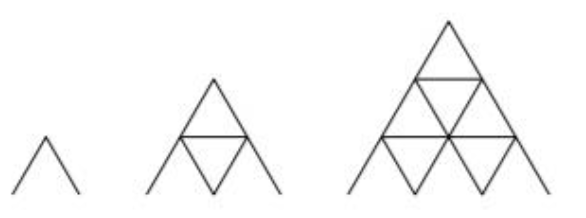
\includegraphics{fig/kaartenhuisje.png}
\caption{Tekening bij opgave \ref{kaartenhuisje}}
\label{fig:kaartenhuisje}
\end{figure}
Voorbeeld: 
\begin{itemize}
\item een kaartenhuisje van 1 verdieping = 2 kaarten
\item een kaartenhuisje van 2 verdiepingen = 7  kaarten
\item een kaartenhuisje van 3 verdiepingen = 15 kaarten
\item een kaartenhuisje van 12 verdiepingen = 222 kaarten
\item een kaartenhuisje van 20 verdiepingen = 610 kaarten
\end{itemize}

\begin{opl}
\begin{lstlisting}[caption={Aantal kaarten nodig om een kaartenhuisje te maken}, label=reckaartenHuisje]

public class Kaartenhuisje {

	public static void main(String[] args) {
		for (int n = 1 ; n <= 20 ; n++)
		System.out.println("Aantal Kaarten nodig voor een kaarten huisje van " + n + 
			" verdieping" + (n == 1 ? " = ": "en = ") + aantalKaarten(n));
	}
	
	private static int aantalKaarten(int n){
		if (n < 1) throw new IllegalArgumentException();
		if (n == 1) return 2;
		else return aantalKaarten(n-1) + (n-1) + 2 * n ;
	}

}
\end{lstlisting}

\end{opl}

\end{oef}


\vspace*{\fill}
\framebox[\textwidth]{\centering\parbox{0.85\textwidth}{\noindent Meer oefenmateriaal nodig? \\\url{http://codingbat.com/java/Recursion-1} \\en \url{http://codingbat.com/java/Recursion-2}.}}